\documentclass{article}\usepackage[]{graphicx}\usepackage[]{color}
%% maxwidth is the original width if it is less than linewidth
%% otherwise use linewidth (to make sure the graphics do not exceed the margin)
\makeatletter
\def\maxwidth{ %
  \ifdim\Gin@nat@width>\linewidth
    \linewidth
  \else
    \Gin@nat@width
  \fi
}
\makeatother

\definecolor{fgcolor}{rgb}{0.345, 0.345, 0.345}
\newcommand{\hlnum}[1]{\textcolor[rgb]{0.686,0.059,0.569}{#1}}%
\newcommand{\hlstr}[1]{\textcolor[rgb]{0.192,0.494,0.8}{#1}}%
\newcommand{\hlcom}[1]{\textcolor[rgb]{0.678,0.584,0.686}{\textit{#1}}}%
\newcommand{\hlopt}[1]{\textcolor[rgb]{0,0,0}{#1}}%
\newcommand{\hlstd}[1]{\textcolor[rgb]{0.345,0.345,0.345}{#1}}%
\newcommand{\hlkwa}[1]{\textcolor[rgb]{0.161,0.373,0.58}{\textbf{#1}}}%
\newcommand{\hlkwb}[1]{\textcolor[rgb]{0.69,0.353,0.396}{#1}}%
\newcommand{\hlkwc}[1]{\textcolor[rgb]{0.333,0.667,0.333}{#1}}%
\newcommand{\hlkwd}[1]{\textcolor[rgb]{0.737,0.353,0.396}{\textbf{#1}}}%
\let\hlipl\hlkwb

\usepackage{framed}
\makeatletter
\newenvironment{kframe}{%
 \def\at@end@of@kframe{}%
 \ifinner\ifhmode%
  \def\at@end@of@kframe{\end{minipage}}%
  \begin{minipage}{\columnwidth}%
 \fi\fi%
 \def\FrameCommand##1{\hskip\@totalleftmargin \hskip-\fboxsep
 \colorbox{shadecolor}{##1}\hskip-\fboxsep
     % There is no \\@totalrightmargin, so:
     \hskip-\linewidth \hskip-\@totalleftmargin \hskip\columnwidth}%
 \MakeFramed {\advance\hsize-\width
   \@totalleftmargin\z@ \linewidth\hsize
   \@setminipage}}%
 {\par\unskip\endMakeFramed%
 \at@end@of@kframe}
\makeatother

\definecolor{shadecolor}{rgb}{.97, .97, .97}
\definecolor{messagecolor}{rgb}{0, 0, 0}
\definecolor{warningcolor}{rgb}{1, 0, 1}
\definecolor{errorcolor}{rgb}{1, 0, 0}
\newenvironment{knitrout}{}{} % an empty environment to be redefined in TeX

\usepackage{alltt}
\usepackage{natbib}
\usepackage[unicode=true]{hyperref}
\usepackage{geometry}
\geometry{tmargin=1in,bmargin=1in,lmargin=1in,rmargin=1in}


\IfFileExists{upquote.sty}{\usepackage{upquote}}{}
\begin{document} 
\title{STAT243-PS4}
\author{Jinhui Xu}
\date{October 2017}

\maketitle

\section{Other students}
I discuss some problems with Xin Shi.  

\section{Question 1}

\subsection{(a)}
There is only one copy. Because we can see that data and input share same address.
\begin{knitrout}
\definecolor{shadecolor}{rgb}{0.969, 0.969, 0.969}\color{fgcolor}\begin{kframe}
\begin{alltt}
\hlstd{x} \hlkwb{<-} \hlnum{1}\hlopt{:}\hlnum{10}
\hlstd{f} \hlkwb{<-} \hlkwa{function}\hlstd{(}\hlkwc{input}\hlstd{)\{}
  \hlkwd{print}\hlstd{(}\hlkwd{.Internal}\hlstd{(}\hlkwd{inspect}\hlstd{(input)))}       \hlcom{#check the address of input}
  \hlstd{data} \hlkwb{<-} \hlstd{input}
  \hlkwd{print}\hlstd{(}\hlkwd{.Internal}\hlstd{(}\hlkwd{inspect}\hlstd{(data)))}        \hlcom{#check the address of data}
        \hlstd{g} \hlkwb{<-} \hlkwa{function}\hlstd{(}\hlkwc{param}\hlstd{)} \hlkwd{return}\hlstd{(param} \hlopt{*} \hlstd{data)}
        \hlkwd{return}\hlstd{(g)}
\hlstd{\}}
\hlstd{data}\hlkwb{<-}\hlnum{100}
\hlstd{myFun} \hlkwb{<-} \hlkwd{f}\hlstd{(x)}
\end{alltt}
\begin{verbatim}
## @117a12880 13 INTSXP g0c4 [NAM(2)] (len=10, tl=0) 1,2,3,4,5,...
##  [1]  1  2  3  4  5  6  7  8  9 10
## @117a12880 13 INTSXP g0c4 [NAM(2)] (len=10, tl=0) 1,2,3,4,5,...
##  [1]  1  2  3  4  5  6  7  8  9 10
\end{verbatim}
\end{kframe}
\end{knitrout}

\subsection{(b)}
The size of the serialized object is doubled. The reason is that R store both input and data even though they have same address.
\begin{knitrout}
\definecolor{shadecolor}{rgb}{0.969, 0.969, 0.969}\color{fgcolor}\begin{kframe}
\begin{alltt}
\hlstd{x} \hlkwb{<-} \hlkwd{rnorm}\hlstd{(}\hlnum{1e5}\hlstd{)}
\hlstd{f} \hlkwb{<-} \hlkwa{function}\hlstd{(}\hlkwc{input}\hlstd{)\{}
  \hlstd{data} \hlkwb{<-} \hlstd{input}
        \hlstd{g} \hlkwb{<-} \hlkwa{function}\hlstd{(}\hlkwc{param}\hlstd{)} \hlkwd{return}\hlstd{(param} \hlopt{*} \hlstd{data)}
        \hlkwd{return}\hlstd{(g)}
\hlstd{\}}
\hlstd{myFun} \hlkwb{<-} \hlkwd{f}\hlstd{(x)}
\hlkwd{object.size}\hlstd{(x)}
\end{alltt}
\begin{verbatim}
## 800040 bytes
\end{verbatim}
\begin{alltt}
\hlkwd{length}\hlstd{(}\hlkwd{serialize}\hlstd{(myFun,}\hlkwa{NULL}\hlstd{))}
\end{alltt}
\begin{verbatim}
## [1] 1606454
\end{verbatim}
\end{kframe}
\end{knitrout}


\subsection{(c)}
When the function contains the command: data=input. myFun can get the value of data even x is removed.
However, when we delete that command, myFun need the value of input of f which means that myFun needs the value of x. So if we rm x, there would be an error.
\begin{knitrout}
\definecolor{shadecolor}{rgb}{0.969, 0.969, 0.969}\color{fgcolor}\begin{kframe}
\begin{alltt}
\hlstd{x} \hlkwb{<-} \hlnum{1}\hlopt{:}\hlnum{10}
\hlstd{f} \hlkwb{<-} \hlkwa{function}\hlstd{(}\hlkwc{data}\hlstd{)\{}
  \hlstd{g} \hlkwb{<-} \hlkwa{function}\hlstd{(}\hlkwc{param}\hlstd{)} \hlkwd{return}\hlstd{(param} \hlopt{*} \hlstd{data)}
  \hlkwd{return}\hlstd{(g)}
\hlstd{\}}
\hlstd{myFun} \hlkwb{<-} \hlkwd{f}\hlstd{(x)}
\hlkwd{rm}\hlstd{(x)}
\hlstd{data} \hlkwb{<-} \hlnum{100}
\hlkwd{myFun}\hlstd{(}\hlnum{3}\hlstd{)}
\end{alltt}


{\ttfamily\noindent\bfseries\color{errorcolor}{\#\# Error in myFun(3): 找不到对象'x'}}\begin{alltt}
\hlkwd{ls}\hlstd{(}\hlkwc{envir}\hlstd{=}\hlkwd{environment}\hlstd{(myFun))}
\end{alltt}
\begin{verbatim}
## [1] "data" "g"
\end{verbatim}
\end{kframe}
\end{knitrout}

\subsection{(d)}
We can use force to force the value of data.
\begin{knitrout}
\definecolor{shadecolor}{rgb}{0.969, 0.969, 0.969}\color{fgcolor}\begin{kframe}
\begin{alltt}
\hlstd{x} \hlkwb{<-} \hlnum{1}\hlopt{:}\hlnum{10}
\hlstd{f} \hlkwb{<-} \hlkwa{function}\hlstd{(}\hlkwc{data}\hlstd{)\{}
  \hlkwd{force}\hlstd{(data)}
  \hlstd{g} \hlkwb{<-} \hlkwa{function}\hlstd{(}\hlkwc{param}\hlstd{)} \hlkwd{return}\hlstd{(param} \hlopt{*} \hlstd{data)}
  \hlkwd{return}\hlstd{(g)}
\hlstd{\}}
\hlstd{myFun} \hlkwb{<-} \hlkwd{f}\hlstd{(x)}
\hlkwd{rm}\hlstd{(x)}
\hlstd{data} \hlkwb{<-} \hlnum{100}
\hlkwd{myFun}\hlstd{(}\hlnum{3}\hlstd{)}
\end{alltt}
\begin{verbatim}
##  [1]  3  6  9 12 15 18 21 24 27 30
\end{verbatim}
\end{kframe}
\end{knitrout}


\section{Question 2}
\subsection{(a)}
When change the a vector of list, I find that the address of the relevant changes and the other one does not change. Therefore, R would create a new vector.
\begin{knitrout}
\definecolor{shadecolor}{rgb}{0.969, 0.969, 0.969}\color{fgcolor}\begin{kframe}
\begin{alltt}
\hlstd{list1}\hlkwb{=}\hlkwd{list}\hlstd{(}\hlkwc{a}\hlstd{=}\hlkwd{rnorm}\hlstd{(}\hlnum{1e5}\hlstd{),}\hlkwc{b}\hlstd{=}\hlkwd{rnorm}\hlstd{(}\hlnum{1e5}\hlstd{))}
\hlkwd{.Internal}\hlstd{(}\hlkwd{inspect}\hlstd{(list1))}
\end{alltt}
\begin{verbatim}
## @12b4f14b0 19 VECSXP g0c2 [NAM(2),ATT] (len=2, tl=0)
##   @10ec8a000 14 REALSXP g0c7 [] (len=100000, tl=0) 0.163302,1.5673,0.59027,-1.25237,-0.657689,...
##   @112188000 14 REALSXP g0c7 [] (len=100000, tl=0) -0.316091,0.271516,1.18125,0.0445575,-1.83643,...
## ATTRIB:
##   @10971f640 02 LISTSXP g0c0 [] 
##     TAG: @103824140 01 SYMSXP g1c0 [MARK,NAM(2),LCK,gp=0x6000] "names" (has value)
##     @12b4f14e8 16 STRSXP g0c2 [] (len=2, tl=0)
##       @103021b98 09 CHARSXP g1c1 [MARK,gp=0x61] [ASCII] [cached] "a"
##       @1032eab98 09 CHARSXP g1c1 [MARK,gp=0x61] [ASCII] [cached] "b"
\end{verbatim}
\begin{alltt}
\hlstd{list1[[}\hlnum{1}\hlstd{]][}\hlnum{1}\hlstd{]}\hlkwb{<-}\hlnum{100}
\hlkwd{.Internal}\hlstd{(}\hlkwd{inspect}\hlstd{(list1))}
\end{alltt}
\begin{verbatim}
## @13d5cb608 19 VECSXP g0c2 [NAM(1),ATT] (len=2, tl=0)
##   @10b52e000 14 REALSXP g0c7 [] (len=100000, tl=0) 100,1.5673,0.59027,-1.25237,-0.657689,...
##   @112188000 14 REALSXP g0c7 [NAM(2)] (len=100000, tl=0) -0.316091,0.271516,1.18125,0.0445575,-1.83643,...
## ATTRIB:
##   @10f603b78 02 LISTSXP g0c0 [] 
##     TAG: @103824140 01 SYMSXP g1c0 [MARK,NAM(2),LCK,gp=0x6000] "names" (has value)
##     @12b4f14e8 16 STRSXP g0c2 [NAM(2)] (len=2, tl=0)
##       @103021b98 09 CHARSXP g1c1 [MARK,gp=0x61] [ASCII] [cached] "a"
##       @1032eab98 09 CHARSXP g1c1 [MARK,gp=0x61] [ASCII] [cached] "b"
\end{verbatim}
\end{kframe}
\end{knitrout}

\subsection{(b)}
According to the adddress of two lists before any change, we know that there is no copy-on-change.When the change is made, only the address of the relevant vector changes. Therefore, only a copy of the relevant vector is made.
\begin{knitrout}
\definecolor{shadecolor}{rgb}{0.969, 0.969, 0.969}\color{fgcolor}\begin{kframe}
\begin{alltt}
\hlstd{list2}\hlkwb{=}\hlkwd{list}\hlstd{(}\hlkwc{a}\hlstd{=}\hlkwd{rnorm}\hlstd{(}\hlnum{1e5}\hlstd{),}\hlkwc{b}\hlstd{=}\hlkwd{rnorm}\hlstd{(}\hlnum{1e5}\hlstd{))}
\hlstd{list2_cp}\hlkwb{=}\hlstd{list2}
\hlkwd{.Internal}\hlstd{(}\hlkwd{inspect}\hlstd{((list2)))}
\end{alltt}
\begin{verbatim}
## @1197c19f8 19 VECSXP g0c2 [NAM(2),ATT] (len=2, tl=0)
##   @1114cf000 14 REALSXP g0c7 [] (len=100000, tl=0) -0.917492,1.34264,0.880094,-0.928486,1.4136,...
##   @112000000 14 REALSXP g0c7 [] (len=100000, tl=0) -1.08646,-0.686031,1.63498,1.22225,-0.340234,...
## ATTRIB:
##   @11841e0b0 02 LISTSXP g0c0 [] 
##     TAG: @103824140 01 SYMSXP g1c0 [MARK,NAM(2),LCK,gp=0x6000] "names" (has value)
##     @1197c1a68 16 STRSXP g0c2 [] (len=2, tl=0)
##       @103021b98 09 CHARSXP g1c1 [MARK,gp=0x61] [ASCII] [cached] "a"
##       @1032eab98 09 CHARSXP g1c1 [MARK,gp=0x61] [ASCII] [cached] "b"
\end{verbatim}
\begin{alltt}
\hlkwd{.Internal}\hlstd{(}\hlkwd{inspect}\hlstd{((list2_cp)))}
\end{alltt}
\begin{verbatim}
## @1197c19f8 19 VECSXP g0c2 [NAM(2),ATT] (len=2, tl=0)
##   @1114cf000 14 REALSXP g0c7 [] (len=100000, tl=0) -0.917492,1.34264,0.880094,-0.928486,1.4136,...
##   @112000000 14 REALSXP g0c7 [] (len=100000, tl=0) -1.08646,-0.686031,1.63498,1.22225,-0.340234,...
## ATTRIB:
##   @11841e0b0 02 LISTSXP g0c0 [] 
##     TAG: @103824140 01 SYMSXP g1c0 [MARK,NAM(2),LCK,gp=0x6000] "names" (has value)
##     @1197c1a68 16 STRSXP g0c2 [] (len=2, tl=0)
##       @103021b98 09 CHARSXP g1c1 [MARK,gp=0x61] [ASCII] [cached] "a"
##       @1032eab98 09 CHARSXP g1c1 [MARK,gp=0x61] [ASCII] [cached] "b"
\end{verbatim}
\begin{alltt}
\hlcom{#the address of list2_cp is same with that of list2}
\hlstd{list2_cp[[}\hlnum{1}\hlstd{]][}\hlnum{1}\hlstd{]}\hlkwb{<-}\hlnum{100}
\hlkwd{.Internal}\hlstd{(}\hlkwd{inspect}\hlstd{(list2_cp))}
\end{alltt}
\begin{verbatim}
## @12b2d0a78 19 VECSXP g0c2 [NAM(1),ATT] (len=2, tl=0)
##   @11140b000 14 REALSXP g0c7 [] (len=100000, tl=0) 100,1.34264,0.880094,-0.928486,1.4136,...
##   @112000000 14 REALSXP g0c7 [NAM(2)] (len=100000, tl=0) -1.08646,-0.686031,1.63498,1.22225,-0.340234,...
## ATTRIB:
##   @14cf41e00 02 LISTSXP g0c0 [] 
##     TAG: @103824140 01 SYMSXP g1c0 [MARK,NAM(2),LCK,gp=0x6000] "names" (has value)
##     @1197c1a68 16 STRSXP g0c2 [NAM(2)] (len=2, tl=0)
##       @103021b98 09 CHARSXP g1c1 [MARK,gp=0x61] [ASCII] [cached] "a"
##       @1032eab98 09 CHARSXP g1c1 [MARK,gp=0x61] [ASCII] [cached] "b"
\end{verbatim}
\begin{alltt}
\hlcom{#after change, we can find only the address of relevant vector changes}
\end{alltt}
\end{kframe}
\end{knitrout}

\subsection{(c)}
Notice the change of address after adding a vector into the second list. The address of two lists becomes different, but two original vectors still have original addresses. So the only change is that the second list creates a new vector while other vectors still share original addresses.
\begin{knitrout}
\definecolor{shadecolor}{rgb}{0.969, 0.969, 0.969}\color{fgcolor}\begin{kframe}
\begin{alltt}
\hlstd{list3}\hlkwb{=}\hlkwd{list}\hlstd{(}\hlkwc{a}\hlstd{=}\hlkwd{list}\hlstd{(}\hlkwd{rnorm}\hlstd{(}\hlnum{1e5}\hlstd{)),}\hlkwc{b}\hlstd{=}\hlkwd{list}\hlstd{(}\hlkwd{rnorm}\hlstd{(}\hlnum{1e5}\hlstd{)))}
\hlstd{list3_cp}\hlkwb{=}\hlstd{list3}
\hlkwd{.Internal}\hlstd{(}\hlkwd{inspect}\hlstd{(list3))}
\end{alltt}
\begin{verbatim}
## @11a704b88 19 VECSXP g0c2 [NAM(2),ATT] (len=2, tl=0)
##   @103dd0d28 19 VECSXP g0c1 [] (len=1, tl=0)
##     @110d00000 14 REALSXP g0c7 [] (len=100000, tl=0) -0.304923,0.11101,0.137074,-0.389024,-0.476274,...
##   @103dd0de8 19 VECSXP g0c1 [] (len=1, tl=0)
##     @11224c000 14 REALSXP g0c7 [] (len=100000, tl=0) 0.380603,-0.357204,-0.230827,0.886193,-0.540597,...
## ATTRIB:
##   @111b98758 02 LISTSXP g0c0 [] 
##     TAG: @103824140 01 SYMSXP g1c0 [MARK,NAM(2),LCK,gp=0x6000] "names" (has value)
##     @11a704c68 16 STRSXP g0c2 [] (len=2, tl=0)
##       @103021b98 09 CHARSXP g1c1 [MARK,gp=0x61] [ASCII] [cached] "a"
##       @1032eab98 09 CHARSXP g1c1 [MARK,gp=0x61] [ASCII] [cached] "b"
\end{verbatim}
\begin{alltt}
\hlkwd{.Internal}\hlstd{(}\hlkwd{inspect}\hlstd{(list3_cp))}
\end{alltt}
\begin{verbatim}
## @11a704b88 19 VECSXP g0c2 [NAM(2),ATT] (len=2, tl=0)
##   @103dd0d28 19 VECSXP g0c1 [] (len=1, tl=0)
##     @110d00000 14 REALSXP g0c7 [] (len=100000, tl=0) -0.304923,0.11101,0.137074,-0.389024,-0.476274,...
##   @103dd0de8 19 VECSXP g0c1 [] (len=1, tl=0)
##     @11224c000 14 REALSXP g0c7 [] (len=100000, tl=0) 0.380603,-0.357204,-0.230827,0.886193,-0.540597,...
## ATTRIB:
##   @111b98758 02 LISTSXP g0c0 [] 
##     TAG: @103824140 01 SYMSXP g1c0 [MARK,NAM(2),LCK,gp=0x6000] "names" (has value)
##     @11a704c68 16 STRSXP g0c2 [] (len=2, tl=0)
##       @103021b98 09 CHARSXP g1c1 [MARK,gp=0x61] [ASCII] [cached] "a"
##       @1032eab98 09 CHARSXP g1c1 [MARK,gp=0x61] [ASCII] [cached] "b"
\end{verbatim}
\begin{alltt}
\hlstd{list3_cp}\hlopt{$}\hlstd{b[[}\hlnum{2}\hlstd{]]}\hlkwb{<-}\hlkwd{rnorm}\hlstd{(}\hlnum{1e5}\hlstd{)}
\hlkwd{.Internal}\hlstd{(}\hlkwd{inspect}\hlstd{(list3_cp))}
\end{alltt}
\begin{verbatim}
## @11a667588 19 VECSXP g0c2 [NAM(1),ATT] (len=2, tl=0)
##   @103dd0d28 19 VECSXP g0c1 [NAM(2)] (len=1, tl=0)
##     @110d00000 14 REALSXP g0c7 [] (len=100000, tl=0) -0.304923,0.11101,0.137074,-0.389024,-0.476274,...
##   @11a6675c0 19 VECSXP g0c2 [] (len=2, tl=0)
##     @11224c000 14 REALSXP g0c7 [NAM(2)] (len=100000, tl=0) 0.380603,-0.357204,-0.230827,0.886193,-0.540597,...
##     @112310000 14 REALSXP g0c7 [NAM(2)] (len=100000, tl=0) 1.05821,0.760135,0.484417,-1.22833,0.813204,...
## ATTRIB:
##   @111cdde98 02 LISTSXP g0c0 [] 
##     TAG: @103824140 01 SYMSXP g1c0 [MARK,NAM(2),LCK,gp=0x6000] "names" (has value)
##     @11a704c68 16 STRSXP g0c2 [NAM(2)] (len=2, tl=0)
##       @103021b98 09 CHARSXP g1c1 [MARK,gp=0x61] [ASCII] [cached] "a"
##       @1032eab98 09 CHARSXP g1c1 [MARK,gp=0x61] [ASCII] [cached] "b"
\end{verbatim}
\end{kframe}
\end{knitrout}

\subsection{(d)}
Object.size is twice large as the result of gc. I guess that it is because two elements of list is stored in the same address, but object.size estimates the size of list equels to sum of size of each element.
\begin{knitrout}
\definecolor{shadecolor}{rgb}{0.969, 0.969, 0.969}\color{fgcolor}\begin{kframe}
\begin{alltt}
\hlkwd{gc}\hlstd{()}
\end{alltt}
\begin{verbatim}
##            used  (Mb) gc trigger  (Mb)  max used  (Mb)
## Ncells  1968924 105.2    3886542 207.6   3886542 207.6
## Vcells 30853507 235.4   97834876 746.5 109412705 834.8
\end{verbatim}
\begin{alltt}
\hlstd{tmp} \hlkwb{<-} \hlkwd{list}\hlstd{()}
\hlstd{x} \hlkwb{<-} \hlkwd{rnorm}\hlstd{(}\hlnum{1e7}\hlstd{)}
\hlstd{tmp[[}\hlnum{1}\hlstd{]]} \hlkwb{<-} \hlstd{x}
\hlstd{tmp[[}\hlnum{2}\hlstd{]]} \hlkwb{<-} \hlstd{x}
\hlkwd{.Internal}\hlstd{(}\hlkwd{inspect}\hlstd{(tmp))}
\end{alltt}
\begin{verbatim}
## @117682c40 19 VECSXP g0c2 [NAM(1)] (len=2, tl=0)
##   @146800000 14 REALSXP g0c7 [NAM(2)] (len=10000000, tl=0) -0.135277,1.27501,-0.777146,0.638026,-1.77064,...
##   @146800000 14 REALSXP g0c7 [NAM(2)] (len=10000000, tl=0) -0.135277,1.27501,-0.777146,0.638026,-1.77064,...
\end{verbatim}
\begin{alltt}
\hlkwd{object.size}\hlstd{(tmp)}
\end{alltt}
\begin{verbatim}
## 160000136 bytes
\end{verbatim}
\begin{alltt}
\hlkwd{gc}\hlstd{()}
\end{alltt}
\begin{verbatim}
##            used  (Mb) gc trigger  (Mb)  max used  (Mb)
## Ncells  1968862 105.2    3886542 207.6   3886542 207.6
## Vcells 30853415 235.4   97834876 746.5 109412705 834.8
\end{verbatim}
\end{kframe}
\end{knitrout}

\section{Question 3}
Notice that in the original code,firstly, the if else is not necessary at all. So I directly calculate q without if else. Secondly I replace three nested for loops with simple computation of vector
\begin{knitrout}
\definecolor{shadecolor}{rgb}{0.969, 0.969, 0.969}\color{fgcolor}\begin{kframe}
\begin{alltt}
\hlstd{ll} \hlkwb{<-} \hlkwa{function}\hlstd{(}\hlkwc{Theta}\hlstd{,} \hlkwc{A}\hlstd{) \{}
  \hlstd{sum.ind} \hlkwb{<-} \hlkwd{which}\hlstd{(A}\hlopt{==}\hlnum{1}\hlstd{,} \hlkwc{arr.ind}\hlstd{=T)}
  \hlstd{logLik} \hlkwb{<-} \hlkwd{sum}\hlstd{(}\hlkwd{log}\hlstd{(Theta[sum.ind]))} \hlopt{-} \hlkwd{sum}\hlstd{(Theta)}
  \hlkwd{return}\hlstd{(logLik)}
\hlstd{\}}
\hlcom{#######################################}
\hlcom{##original code########################}
\hlstd{oneUpdate} \hlkwb{<-} \hlkwa{function}\hlstd{(}\hlkwc{A}\hlstd{,} \hlkwc{n}\hlstd{,} \hlkwc{K}\hlstd{,} \hlkwc{theta.old}\hlstd{,} \hlkwc{thresh} \hlstd{=} \hlnum{0.1}\hlstd{) \{}
  \hlstd{theta.old1} \hlkwb{<-} \hlstd{theta.old}
  \hlstd{Theta.old} \hlkwb{<-} \hlstd{theta.old} \hlopt \hlkwd{t}\hlstd{(theta.old)}
  \hlstd{L.old} \hlkwb{<-} \hlkwd{ll}\hlstd{(Theta.old, A)}
  \hlstd{q} \hlkwb{<-} \hlkwd{array}\hlstd{(}\hlnum{0}\hlstd{,} \hlkwc{dim} \hlstd{=} \hlkwd{c}\hlstd{(n, n, K))}
\hlcom{##############the following part would be revised}
  \hlkwa{for} \hlstd{(i} \hlkwa{in} \hlnum{1}\hlopt{:}\hlstd{n) \{}
    \hlkwa{for} \hlstd{(j} \hlkwa{in} \hlnum{1}\hlopt{:}\hlstd{n) \{}
      \hlkwa{for} \hlstd{(z} \hlkwa{in} \hlnum{1}\hlopt{:}\hlstd{K) \{}
        \hlkwa{if} \hlstd{(theta.old[i, z]}\hlopt{*}\hlstd{theta.old[j, z]} \hlopt{==} \hlnum{0}\hlstd{)\{}
        \hlstd{q[i, j, z]} \hlkwb{<-} \hlnum{0} \hlstd{\}} \hlkwa{else} \hlstd{\{}
           \hlstd{q[i, j, z]} \hlkwb{<-} \hlstd{theta.old[i, z]}\hlopt{*}\hlstd{theta.old[j, z]} \hlopt{/}\hlstd{Theta.old[i, j]}
         \hlstd{\}}
       \hlstd{\}}
     \hlstd{\}}
  \hlstd{\}}
\hlcom{################}
  \hlstd{theta.new} \hlkwb{<-} \hlstd{theta.old}
  \hlkwa{for} \hlstd{(z} \hlkwa{in} \hlnum{1}\hlopt{:}\hlstd{K) \{}
  \hlstd{theta.new[,z]} \hlkwb{<-} \hlkwd{rowSums}\hlstd{(A}\hlopt{*}\hlstd{q[,,z])}\hlopt{/}\hlkwd{sqrt}\hlstd{(}\hlkwd{sum}\hlstd{(A}\hlopt{*}\hlstd{q[,,z]))}
  \hlstd{\}}
  \hlstd{Theta.new} \hlkwb{<-} \hlstd{theta.new} \hlopt \hlkwd{t}\hlstd{(theta.new)}
  \hlstd{L.new} \hlkwb{<-} \hlkwd{ll}\hlstd{(Theta.new, A)}
      \hlstd{converge.check} \hlkwb{<-} \hlkwd{abs}\hlstd{(L.new} \hlopt{-} \hlstd{L.old)} \hlopt{<} \hlstd{thresh}
  \hlstd{theta.new} \hlkwb{<-} \hlstd{theta.new}\hlopt{/}\hlkwd{rowSums}\hlstd{(theta.new)}
  \hlkwd{return}\hlstd{(}\hlkwd{list}\hlstd{(}\hlkwc{theta} \hlstd{= theta.new,} \hlkwc{loglik} \hlstd{= L.new,}\hlkwc{converged} \hlstd{= converge.check))}
\hlstd{\}}

\hlcom{#######################################}
\hlcom{##revised code#########################}
\hlstd{oneUpdate_new} \hlkwb{<-} \hlkwa{function}\hlstd{(}\hlkwc{A}\hlstd{,} \hlkwc{n}\hlstd{,} \hlkwc{K}\hlstd{,} \hlkwc{theta.old}\hlstd{,} \hlkwc{thresh} \hlstd{=} \hlnum{0.1}\hlstd{) \{}
  \hlstd{theta.old1} \hlkwb{<-} \hlstd{theta.old}
  \hlstd{Theta.old} \hlkwb{<-} \hlstd{theta.old} \hlopt \hlkwd{t}\hlstd{(theta.old)}
  \hlstd{L.old} \hlkwb{<-} \hlkwd{ll}\hlstd{(Theta.old, A)}
  \hlstd{q} \hlkwb{<-} \hlkwd{array}\hlstd{(}\hlnum{0}\hlstd{,} \hlkwc{dim} \hlstd{=} \hlkwd{c}\hlstd{(n, n, K))}
\hlcom{####################begin.revised part}
  \hlkwa{for} \hlstd{(z} \hlkwa{in} \hlnum{1}\hlopt{:}\hlstd{K) \{}
       \hlstd{q[ , , z]} \hlkwb{<-} \hlstd{theta.old[, z]}\hlopt\hlkwd{t}\hlstd{(theta.old[ , z])} \hlopt{/}\hlstd{Theta.old}
  \hlstd{\}}
\hlcom{####################end.revised part}
  \hlstd{theta.new} \hlkwb{<-} \hlstd{theta.old}
  \hlkwa{for} \hlstd{(z} \hlkwa{in} \hlnum{1}\hlopt{:}\hlstd{K) \{}
  \hlstd{theta.new[,z]} \hlkwb{<-} \hlkwd{rowSums}\hlstd{(A}\hlopt{*}\hlstd{q[,,z])}\hlopt{/}\hlkwd{sqrt}\hlstd{(}\hlkwd{sum}\hlstd{(A}\hlopt{*}\hlstd{q[,,z]))}
  \hlstd{\}}
  \hlstd{Theta.new} \hlkwb{<-} \hlstd{theta.new} \hlopt \hlkwd{t}\hlstd{(theta.new)}
  \hlstd{L.new} \hlkwb{<-} \hlkwd{ll}\hlstd{(Theta.new, A)}
      \hlstd{converge.check} \hlkwb{<-} \hlkwd{abs}\hlstd{(L.new} \hlopt{-} \hlstd{L.old)} \hlopt{<} \hlstd{thresh}
  \hlstd{theta.new} \hlkwb{<-} \hlstd{theta.new}\hlopt{/}\hlkwd{rowSums}\hlstd{(theta.new)}
  \hlkwd{return}\hlstd{(}\hlkwd{list}\hlstd{(}\hlkwc{theta} \hlstd{= theta.new,} \hlkwc{loglik} \hlstd{= L.new,}\hlkwc{converged} \hlstd{= converge.check))}
\hlstd{\}}
\hlcom{# initialize the parameters at random starting values}
\hlstd{temp} \hlkwb{<-} \hlkwd{matrix}\hlstd{(}\hlkwd{runif}\hlstd{(n}\hlopt{*}\hlstd{K), n, K)}
\hlstd{theta.init} \hlkwb{<-} \hlstd{temp}\hlopt{/}\hlkwd{rowSums}\hlstd{(temp)}
\hlcom{#compare the time used }
\hlkwd{system.time}\hlstd{(out} \hlkwb{<-} \hlkwd{oneUpdate}\hlstd{(A, n, K, theta.init))}
\hlkwd{system.time}\hlstd{(out_new} \hlkwb{<-} \hlkwd{oneUpdate_new}\hlstd{(A, n, K, theta.init))}
\hlkwd{all.equal}\hlstd{(out,out_new)}
\end{alltt}
\end{kframe}
\end{knitrout}
The results are same while the time used by revised code decreases.

\section{Question 4}
Notice that in the function FYKD, the for loop is aim to generate vector x. However, the algorithm only need the first k value of vector x. So we can only calculate that part rather than entire vector.
\begin{knitrout}
\definecolor{shadecolor}{rgb}{0.969, 0.969, 0.969}\color{fgcolor}\begin{kframe}
\begin{alltt}
\hlstd{PIKK} \hlkwb{<-} \hlkwa{function}\hlstd{(}\hlkwc{x}\hlstd{,} \hlkwc{k}\hlstd{) \{}
\hlstd{x[}\hlkwd{sort}\hlstd{(}\hlkwd{runif}\hlstd{(}\hlkwd{length}\hlstd{(x)),} \hlkwc{index.return} \hlstd{=} \hlnum{TRUE}\hlstd{)}\hlopt{$}\hlstd{ix[}\hlnum{1}\hlopt{:}\hlstd{k]]}
\hlstd{\}}
\hlstd{FYKD} \hlkwb{<-} \hlkwa{function}\hlstd{(}\hlkwc{x}\hlstd{,} \hlkwc{k}\hlstd{) \{}
  \hlstd{n} \hlkwb{<-} \hlkwd{length}\hlstd{(x)}
\hlcom{#in the original code , the following code is to generate entire n values in vector x}
  \hlkwa{for}\hlstd{(i} \hlkwa{in} \hlnum{1}\hlopt{:}\hlstd{n) \{}
     \hlstd{j} \hlkwb{=} \hlkwd{sample}\hlstd{(i}\hlopt{:}\hlstd{n,} \hlnum{1}\hlstd{)}
     \hlstd{tmp} \hlkwb{<-} \hlstd{x[i]}
     \hlstd{x[i]} \hlkwb{<-} \hlstd{x[j]}
     \hlstd{x[j]} \hlkwb{<-} \hlstd{tmp}
  \hlstd{\}}
\hlkwd{return}\hlstd{(x[}\hlnum{1}\hlopt{:}\hlstd{k])}  \hlcom{# while we only need first k values }
\hlstd{\}}

\hlcom{#so revised code do not calculate the latter part of the vector}
\hlstd{FYKD_new} \hlkwb{<-} \hlkwa{function}\hlstd{(}\hlkwc{x}\hlstd{,} \hlkwc{k}\hlstd{) \{}
  \hlstd{n} \hlkwb{<-} \hlkwd{length}\hlstd{(x)}
  \hlkwa{for}\hlstd{(i} \hlkwa{in} \hlnum{1}\hlopt{:}\hlstd{k) \{}
     \hlstd{j} \hlkwb{=} \hlkwd{sample}\hlstd{(i}\hlopt{:}\hlstd{n,} \hlnum{1}\hlstd{)}
     \hlstd{tmp} \hlkwb{<-} \hlstd{x[i]}
     \hlstd{x[i]} \hlkwb{<-} \hlstd{x[j]}
     \hlstd{x[j]} \hlkwb{<-} \hlstd{tmp}
  \hlstd{\}}
\hlkwd{return}\hlstd{(x[}\hlnum{1}\hlopt{:}\hlstd{k])}
\hlstd{\}}
\end{alltt}
\end{kframe}
\end{knitrout}

Then compare the revised code and original code in term of time needed to calculate the result.
\begin{knitrout}
\definecolor{shadecolor}{rgb}{0.969, 0.969, 0.969}\color{fgcolor}\begin{kframe}
\begin{alltt}
\hlcom{####calculate time from different value of n,k. Find that microbenchmark does 100 simulations.}
\hlstd{x}\hlkwb{=}\hlkwd{rnorm}\hlstd{(}\hlnum{10000}\hlstd{)}
\hlstd{FYKD_newtime_10000_500}\hlkwb{<-}\hlkwd{microbenchmark}\hlstd{(}\hlkwd{FYKD_new}\hlstd{(x,}\hlnum{500}\hlstd{))}\hlopt{$}\hlstd{time}
\hlstd{FYKD_time_10000_500}\hlkwb{<-}\hlkwd{microbenchmark}\hlstd{(}\hlkwd{FYKD}\hlstd{(x,}\hlnum{500}\hlstd{))}\hlopt{$}\hlstd{time}
\hlstd{FYKD_newtime_10000_100}\hlkwb{<-}\hlkwd{microbenchmark}\hlstd{(}\hlkwd{FYKD_new}\hlstd{(x,}\hlnum{100}\hlstd{))}\hlopt{$}\hlstd{time}
\hlstd{FYKD_time_10000_100}\hlkwb{<-}\hlkwd{microbenchmark}\hlstd{(}\hlkwd{FYKD}\hlstd{(x,}\hlnum{100}\hlstd{))}\hlopt{$}\hlstd{time}
\hlstd{x}\hlkwb{=}\hlkwd{rnorm}\hlstd{(}\hlnum{20000}\hlstd{)}
\hlstd{FYKD_newtime_20000_500}\hlkwb{<-}\hlkwd{microbenchmark}\hlstd{(}\hlkwd{FYKD_new}\hlstd{(x,}\hlnum{500}\hlstd{))}\hlopt{$}\hlstd{time}
\hlstd{FYKD_time_20000_500}\hlkwb{<-}\hlkwd{microbenchmark}\hlstd{(}\hlkwd{FYKD}\hlstd{(x,}\hlnum{500}\hlstd{))}\hlopt{$}\hlstd{time}
\hlstd{FYKD_newtime_20000_1000}\hlkwb{<-}\hlkwd{microbenchmark}\hlstd{(}\hlkwd{FYKD_new}\hlstd{(x,}\hlnum{1000}\hlstd{))}\hlopt{$}\hlstd{time}
\hlstd{FYKD_time_20000_1000}\hlkwb{<-}\hlkwd{microbenchmark}\hlstd{(}\hlkwd{FYKD}\hlstd{(x,}\hlnum{1000}\hlstd{))}\hlopt{$}\hlstd{time}
\end{alltt}
\end{kframe}
\end{knitrout}

\begin{knitrout}
\definecolor{shadecolor}{rgb}{0.969, 0.969, 0.969}\color{fgcolor}\begin{kframe}
\begin{alltt}
\hlcom{#####create dataframe needed to do a boxplot }
\hlstd{data1}\hlkwb{=}\hlkwd{cbind}\hlstd{(}\hlkwd{rep}\hlstd{(}\hlstr{'n10000_k500'}\hlstd{,}\hlnum{100}\hlstd{),}\hlkwd{rep}\hlstd{(}\hlstr{'FYKD_new'}\hlstd{,}\hlnum{100}\hlstd{),FYKD_newtime_10000_500)}
\hlstd{data2}\hlkwb{=}\hlkwd{cbind}\hlstd{(}\hlkwd{rep}\hlstd{(}\hlstr{'n10000_k500'}\hlstd{,}\hlnum{100}\hlstd{),}\hlkwd{rep}\hlstd{(}\hlstr{'FYKD'}\hlstd{,}\hlnum{100}\hlstd{),FYKD_time_10000_500)}
\hlstd{data3}\hlkwb{=}\hlkwd{cbind}\hlstd{(}\hlkwd{rep}\hlstd{(}\hlstr{'n10000_k100'}\hlstd{,}\hlnum{100}\hlstd{),}\hlkwd{rep}\hlstd{(}\hlstr{'FYKD_new'}\hlstd{,}\hlnum{100}\hlstd{),FYKD_newtime_10000_100)}
\hlstd{data4}\hlkwb{=}\hlkwd{cbind}\hlstd{(}\hlkwd{rep}\hlstd{(}\hlstr{'n10000_k100'}\hlstd{,}\hlnum{100}\hlstd{),}\hlkwd{rep}\hlstd{(}\hlstr{'FYKD'}\hlstd{,}\hlnum{100}\hlstd{),FYKD_time_10000_100)}
\hlstd{data5}\hlkwb{=}\hlkwd{cbind}\hlstd{(}\hlkwd{rep}\hlstd{(}\hlstr{'n20000_k500'}\hlstd{,}\hlnum{100}\hlstd{),}\hlkwd{rep}\hlstd{(}\hlstr{'FYKD_new'}\hlstd{,}\hlnum{100}\hlstd{),FYKD_newtime_20000_500)}
\hlstd{data6}\hlkwb{=}\hlkwd{cbind}\hlstd{(}\hlkwd{rep}\hlstd{(}\hlstr{'n20000_k500'}\hlstd{,}\hlnum{100}\hlstd{),}\hlkwd{rep}\hlstd{(}\hlstr{'FYKD'}\hlstd{,}\hlnum{100}\hlstd{),FYKD_time_20000_500)}
\hlstd{data7}\hlkwb{=}\hlkwd{cbind}\hlstd{(}\hlkwd{rep}\hlstd{(}\hlstr{'n20000_k1000'}\hlstd{,}\hlnum{100}\hlstd{),}\hlkwd{rep}\hlstd{(}\hlstr{'FYKD_new'}\hlstd{,}\hlnum{100}\hlstd{),FYKD_newtime_20000_1000)}
\hlstd{data8}\hlkwb{=}\hlkwd{cbind}\hlstd{(}\hlkwd{rep}\hlstd{(}\hlstr{'n20000_k1000'}\hlstd{,}\hlnum{100}\hlstd{),}\hlkwd{rep}\hlstd{(}\hlstr{'FYKD'}\hlstd{,}\hlnum{100}\hlstd{),FYKD_time_20000_1000)}
\hlstd{data}\hlkwb{=}\hlkwd{rbind}\hlstd{(data1,data2,data3,data4,data5,data6,data7,data8)}
\hlkwd{colnames}\hlstd{(data)}\hlkwb{<-}\hlkwd{c}\hlstd{(}\hlstr{'nkvalue'}\hlstd{,}\hlstr{'algorithm'}\hlstd{,}\hlstr{'time'}\hlstd{)}
\hlstd{data}\hlkwb{=}\hlkwd{as.data.frame}\hlstd{(data)}
\hlstd{data[,}\hlnum{3}\hlstd{]}\hlkwb{=}\hlkwd{as.numeric}\hlstd{(}\hlkwd{as.character}\hlstd{(data[,}\hlnum{3}\hlstd{]))} \hlcom{#change factor to numeric}
\end{alltt}
\end{kframe}
\end{knitrout}

\begin{knitrout}
\definecolor{shadecolor}{rgb}{0.969, 0.969, 0.969}\color{fgcolor}\begin{kframe}
\begin{alltt}
\hlcom{###do a boxplot}
\hlstd{p}\hlkwb{<-}\hlkwd{ggplot}\hlstd{(}\hlkwc{data}\hlstd{=data,} \hlkwd{aes}\hlstd{(}\hlkwc{x}\hlstd{=nkvalue,}\hlkwc{y}\hlstd{=time))}\hlopt{+}\hlkwd{geom_boxplot}\hlstd{(}\hlkwd{aes}\hlstd{(}\hlkwc{fill}\hlstd{=algorithm))}
\hlstd{p}\hlopt{+} \hlkwd{facet_wrap}\hlstd{(}\hlopt{~} \hlstd{nkvalue,} \hlkwc{scales}\hlstd{=}\hlstr{"free"}\hlstd{)}
\end{alltt}
\end{kframe}
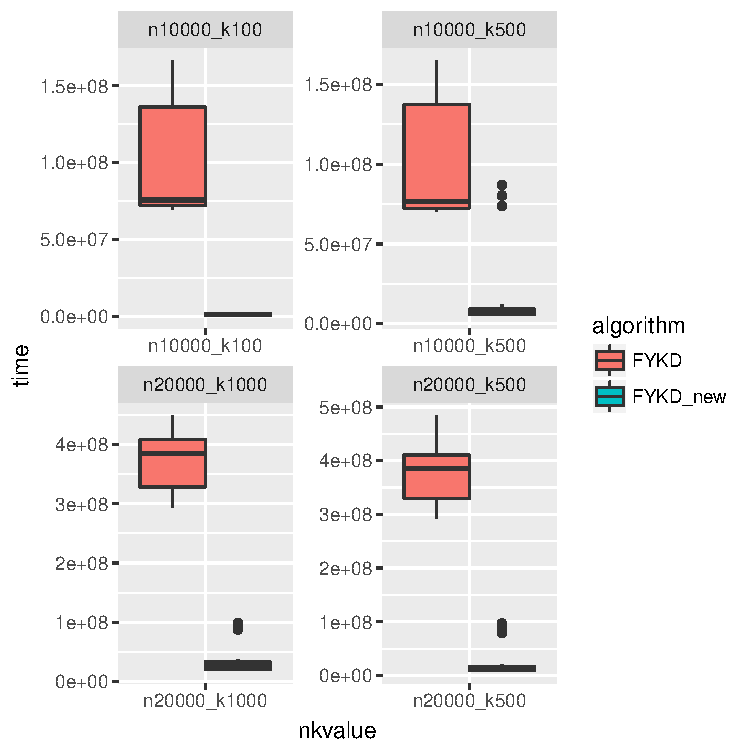
\includegraphics[width=\maxwidth]{figure/r-chunk13-1} 

\end{knitrout}
It is obviously that new algoritnm costs much less time. To view a clearer plot, I do a log function on data.
\begin{knitrout}
\definecolor{shadecolor}{rgb}{0.969, 0.969, 0.969}\color{fgcolor}\begin{kframe}
\begin{alltt}
\hlcom{###go a log function on data[,3],and do boxplot on data_log}
\hlstd{data_log}\hlkwb{=}\hlstd{data}
\hlstd{data_log[,}\hlnum{3}\hlstd{]}\hlkwb{=}\hlkwd{log}\hlstd{(data[,}\hlnum{3}\hlstd{])}
\hlstd{p}\hlkwb{<-}\hlkwd{ggplot}\hlstd{(}\hlkwc{data}\hlstd{=data_log,} \hlkwd{aes}\hlstd{(}\hlkwc{x}\hlstd{=nkvalue,}\hlkwc{y}\hlstd{=time))}\hlopt{+}\hlkwd{geom_boxplot}\hlstd{(}\hlkwd{aes}\hlstd{(}\hlkwc{fill}\hlstd{=algorithm))}
\hlstd{p}\hlopt{+} \hlkwd{facet_wrap}\hlstd{(}\hlopt{~} \hlstd{nkvalue,} \hlkwc{scales}\hlstd{=}\hlstr{"free"}\hlstd{)}
\end{alltt}
\end{kframe}
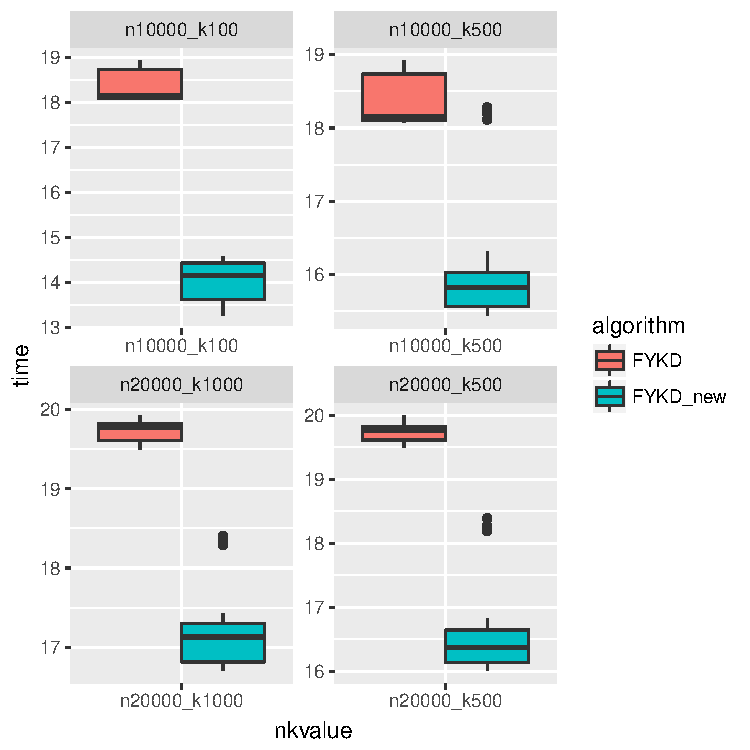
\includegraphics[width=\maxwidth]{figure/r-chunk14-1} 

\end{knitrout}

We can find that revised algorithm performs better as n increases or k decreases.
\end{document}
